\subsection{slow simulator}

笔者参与工作的最新版本的slow simulator可以在笔者的Github上找到。整个slow simulator的工作流程如图\ref{fig:Simulator_flow}所示。
\begin{figure}[htb]
    \begin{center}
    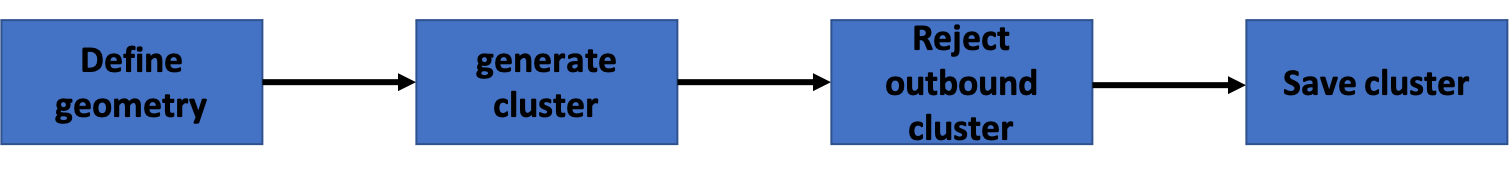
\includegraphics[width=0.7\textwidth,clip]{figures/Chapter3/Simulator_flow.png}
    \end{center}
    \caption[sTGC slow simulator 工作流程示意图]{sTGC slow simulator 工作流程示意图}
    \label{fig:Simulator_flow}
\end{figure}

首先是对整个前向窄隙室径迹探测器的几何结构的定义。最终五边形构型的窄隙室模组的读出条分布如图\ref{fig:sTGC_PCB}所示,其中左图为沿着水平或者竖直方向读出条的分布,右图为沿着对角线方向的读出条的分布。可以看到整个读出条在水平和竖直方向上被分成了三组,在沿对角线方向上被分成了两组。因为这些读出条是通过不同的通道读出,所以在模拟的时候这些不同的组内的信号响应要分别进行模拟。在初版的simulator当中,对cluster响应信号的模拟是因为在探测器当中可以产生一个二维的高斯分布并往X与Y两个方向进行投影,其中高斯分布使用史迎迎在山大测试当中得到的信号宽度分布作为输入。但在后来的讨论当中发现,实际测试得到的高斯分布并不是一个二维的信号分布在一维上的投影,而是在一维方向上直接得到的。所以二维的高斯分布在模拟实际的信号响应的时候会有偏差,在之后的版本中对信号的模拟从二维的高斯分布调整成为了沿着垂直于读出条方向上的一维高斯分布,如图\ref{fig:Simulator_Cluster}右图所示。

\begin{figure}[htb]
    \centering
    \begin{subfigure}[b]{0.45\textwidth}
        \centering
        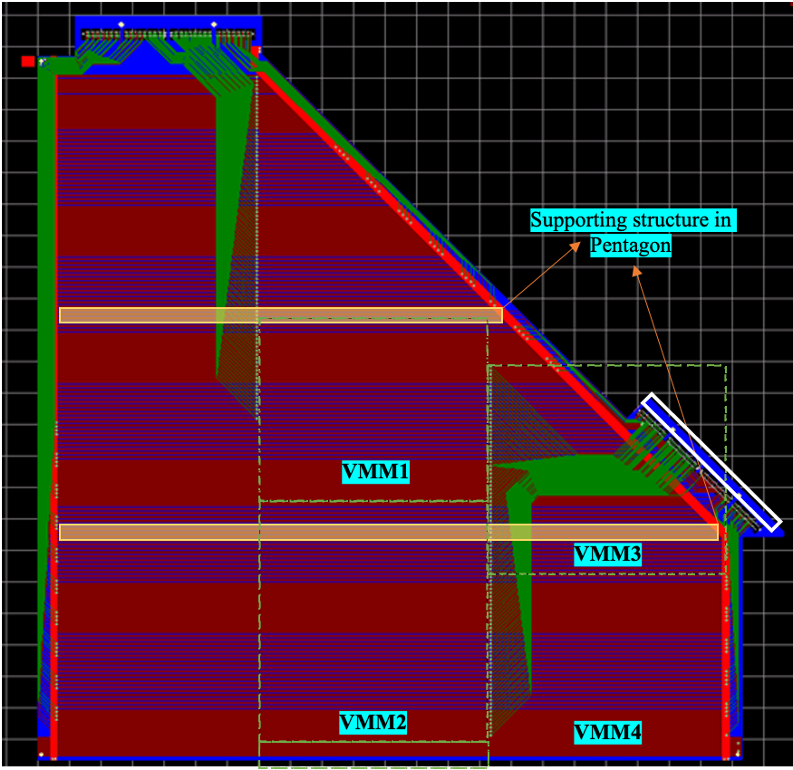
\includegraphics[width=\textwidth,clip]{figures/Chapter3/sTGC_PCB_HV.png}
        \caption{}
        \label{fig:sTGC_PCB_HV}
    \end{subfigure}
    \hfill
    \begin{subfigure}[b]{0.45\textwidth}
        \centering
        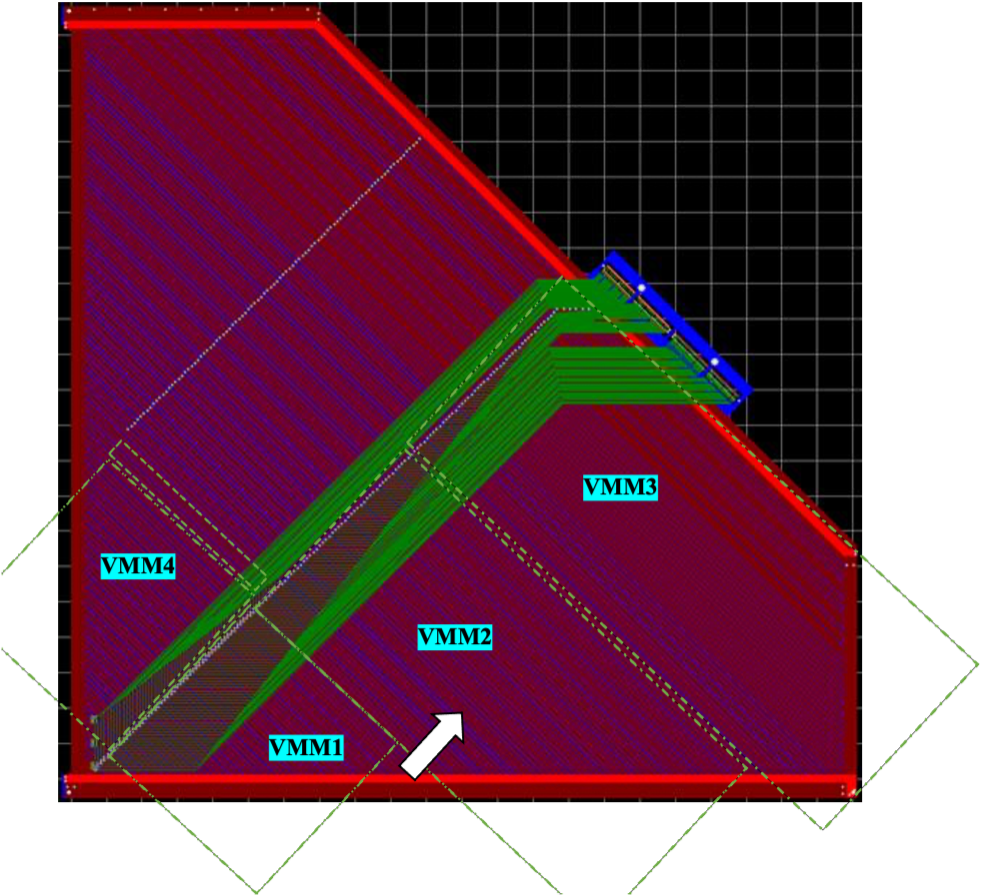
\includegraphics[width=\textwidth,clip]{figures/Chapter3/sTGC_PCB_Diag.png}
        \caption{}
        \label{fig:sTGC_PCB_Diag}
    \end{subfigure}
    \caption[五边形构型sTGC模组读出条分布示意图]{\ref{fig:sTGC_PCB_HV}读出条为水平或者竖直方向上的分布示意图。\ref{fig:sTGC_PCB_Diag}为沿对角线方向的读出条的分布示意图。}
       \label{fig:sTGC_PCB}
\end{figure}
\begin{figure}[htb]
    \begin{center}
    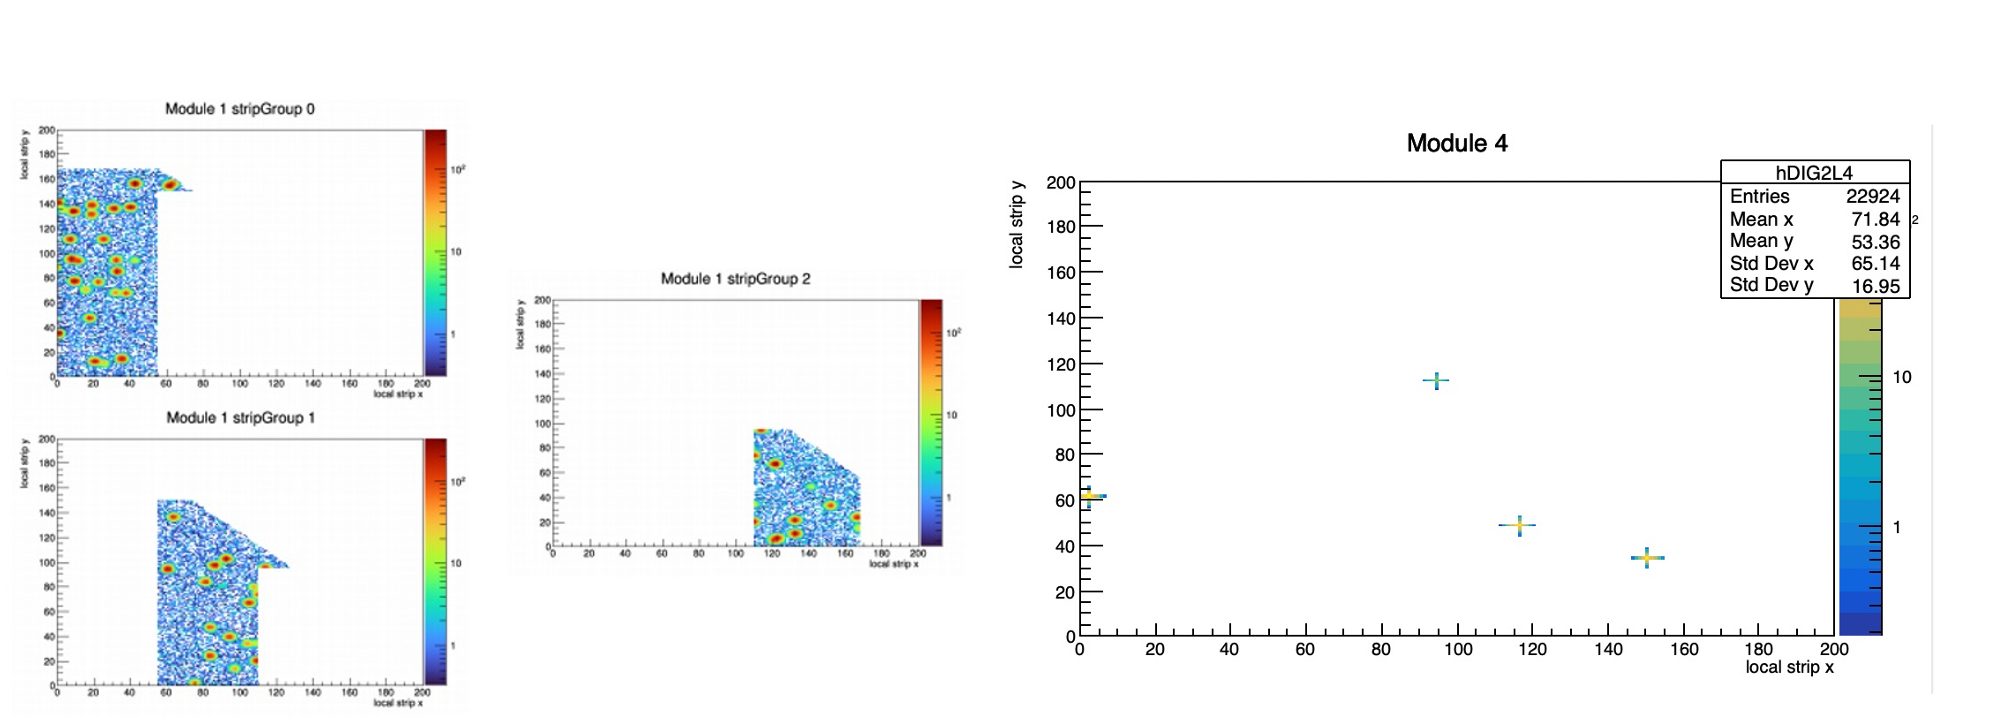
\includegraphics[width=0.85\textwidth,clip]{figures/Chapter3/Simulator_Cluster.png}
    \end{center}
    \caption[slow simulator 对cluster响应的模拟]{slow simulator 对cluster响应的模拟。左图为初版simulator对cluster响应的模拟,此时认为cluster在探测器当中产生的分布为二维的高斯分布,在没有cluster位置的bin当中的content为对噪音的模拟。右图为最新的simulator当中对cluster信号的模拟,已经改为两个方向上的高斯分布。右图当中没有对噪音的模拟。}
    \label{fig:Simulator_Cluster}
\end{figure}

在模拟的时候如何模拟打在边界的cluster是一个需要注意的问题。从图\ref{fig:sTGC_PCB}中可以看到,因为五边形构型的原因,读出条的分布并不是三组完全平行且每组当中所有读出条长度相同的三组读出条,而是在同一个方向有交界的三组。这样当一个粒子击中在读出条的边界的时候实际上会在两组读出条中同时产生信号。在模拟的时候需要注意当一个cluster在读出条组的边界时在不同组的响应问题。同时在cluster finder进行cluster重建的时候也要对这种事例进行额外的处理。这部分将会在cluster finder的部分进行详细介绍。

simulator在编写时遇到的最后一个问题是如何处理cluster在沿对角线方向上的响应。当我们在模拟沿着X和Y方向上读出条响应的时候,只需要对坐标进行简单的投影就可以得到cluster和每一个响应的读出条的坐标。但因为沿着对角线方向的读出条是垂直于每个象限的角平分线的,cluster的坐标需要沿着逆时针或者顺时针旋转$45^{\circ}$后再用来计算应该对应哪些读出条响应。这个转动和计算也在simulator中添加了专门的函数进行处理。

当这些问题被解决好之后slow simulator就可以比较好的模拟探测器对粒子击中的响应。之后的cluster finder的编写工作就利用slow simulator的模拟数据进行初步测试。